% =====================================================================
%  RESULTADOS (versión recortada, para comparar con
%  capitulos/08-resultados.tex)
%
%  Recorte del 2026-10-25:
%   - «Ancho del intervalo de confianza» sale de las limitaciones: repetía lo
%     dicho con la tabla de la campaña en simulación.
%   - La llegada sin flexómetro se explica una sola vez, en la última
%     limitación; las condiciones de las pruebas solo remiten a ella.
%   - Voz de los autores donde se interpreta un resultado; registro
%     impersonal en lo que se reporta.
%   - Figuras y tablas con [htbp].
%  Ninguna cifra de resultado sale del capítulo.
% =====================================================================
\chapter{Resultados}
\label{cap:resultados}

Las dos campañas, en simulación y con los vehículos, se reportan por separado. La de
simulación produce la evidencia estadística, y la de los vehículos demuestra que
el sistema opera sobre la plataforma real.

% ---------------------------------------------------------------------
\section{Evaluación en simulación}
\label{sec:res-sim}

La campaña corrió treinta misiones sorteadas: quince de control, con origen y
destino en el mismo piso, y quince entre pisos, con un relevo. El analizador la
dictaminó válida, sin ningún descarte, frente a un máximo admitido del 20~\%.

\subsection{Tasa de éxito}

Una misión es exitosa si la pose final queda a 0,25~m o menos del destino,
medida contra la odometría y no contra el resultado de Nav2, y si llega a
completarse sin pasar por fallo. La tabla~\ref{tab:exito} da la tasa de cada grupo
con su intervalo de confianza de Wilson al 95~\% \autocite{wilson1927probable}.

\begin{table}[htbp]
  \caption{Tasa de éxito de la campaña en simulación, con intervalo de confianza
    de Wilson al 95~\%.}
  \label{tab:exito}
  \begin{tabular}{@{}lcccc@{}}
    \toprule
    \textbf{Misiones} & \textbf{n} & \textbf{éxitos} & \textbf{tasa} & \textbf{intervalo al 95~\%} \\ \midrule
    Campaña completa & 30 & 26 & 86,7 \% & 70,3 -- 94,7 \% \\
    Mismo piso (control) & 15 & 12 & 80,0 \% & 54,8 -- 93,0 \% \\
    Entre pisos, con relevo & 15 & 14 & 93,3 \% & 70,2 -- 98,8 \% \\ \bottomrule
  \end{tabular}
\end{table}

Lo que podemos afirmar es que la tasa de éxito supera el 70~\%, no que sea del
86,7~\%. Con treinta misiones el intervalo mide 24 puntos porcentuales de ancho, y
ese límite es de diseño: solo se reduce con más muestra. El 86,7~\% es el
estimador puntual y se reporta siempre junto a su intervalo. Los intervalos de
los dos grupos se solapan, así que la comparación entre ellos no sostiene ninguna
conclusión, aunque el estimador puntual apunte en contra de la intuición: las
misiones con relevo salieron mejor que las de control.

\subsection{Causa común de los cuatro fallos}

Las cuatro misiones fallidas quedaron a 0,295, 0,284, 0,311 y 0,347~m del
destino, frente a una tolerancia de 0,25~m. Las cuatro se quedaron cortas:
ninguna se pasó del destino ni terminó en otro sitio. Los cuatro fallos se deben
al límite de precisión de la aproximación final, y ninguno a la coordinación. El
error de llegada del conjunto tiene una mediana de 0,106~m y va de 0,019 a
0,347~m.

\subsection{Tiempo de respuesta y tiempo de asignación}

El tiempo de respuesta se reporta por escalones, y no con media y desviación, por
una razón de instrumento (tabla~\ref{tab:respuesta}).

\begin{table}[htbp]
  \caption{Tiempo de respuesta de las treinta misiones, en escalones del reloj de
    la simulación.}
  \label{tab:respuesta}
  \begin{tabular}{@{}lcccc@{}}
    \toprule
    \textbf{Tiempo de respuesta} & 0,1 s & 0,2 s & 0,3 s & 0,4 s \\ \midrule
    Misiones & 10 & 15 & 4 & 1 \\ \bottomrule
  \end{tabular}
\end{table}

Los cuatro valores son múltiplos exactos de 100~ms, el paso con que avanza el
reloj de la simulación, y la resolución del instrumento vale entre el 25~\% y el
100~\% de la magnitud medida. Una mediana de 0,2~s significa «uno o dos pasos del
reloj», no «doscientos milisegundos», y dar media y desviación sugeriría una
precisión que el reloj no entrega. Lo que sí se sostiene es la cota, que además es
lo que le importa a un usuario: el robot arranca en menos de medio segundo.

El tiempo de asignación quedó por debajo de 100~ms en las treinta misiones,
varios órdenes de magnitud por debajo de un paso del reloj. Por eso se
caracterizó aparte, en un banco de pruebas con el reloj del sistema: mediana
entre 154 y 175~\textmu s y máximo de 306~\textmu s. La
figura~\ref{fig:simulacion} muestra una misión de la campaña.

\begin{figure}[htbp]
  \centering
  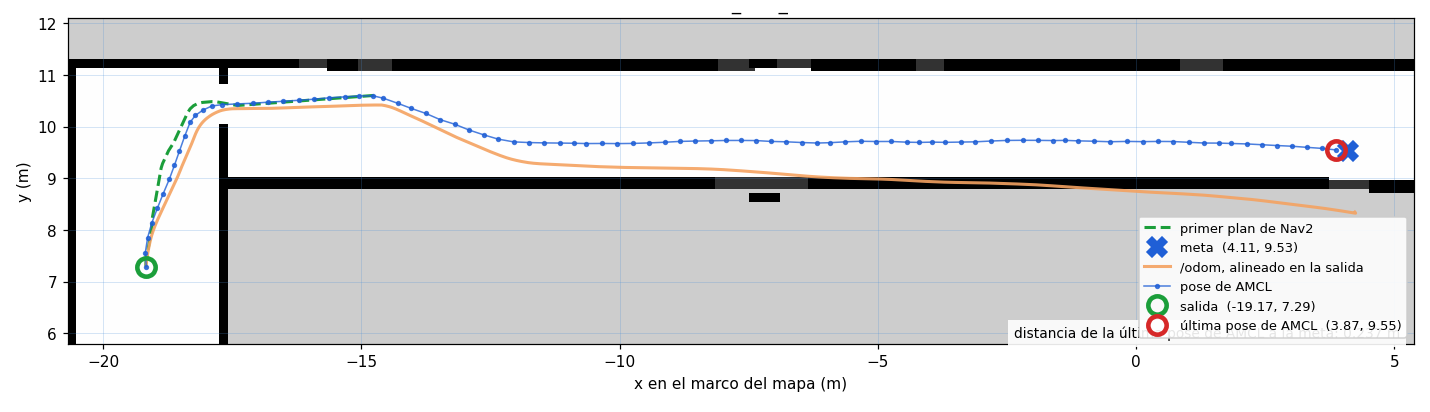
\includegraphics[width=\textwidth]{imagenes/corrida_simulacion.png}
  \caption{Una misión de la campaña en simulación. Se superponen el primer plan
    que calcula el navegador, la pose estimada a lo largo del recorrido y la
    odometría cruda. La separación creciente entre las dos últimas es la deriva
    que la localización corrige contra el mapa.}
  \label{fig:simulacion}
\end{figure}

% ---------------------------------------------------------------------
\section{Evaluación con los vehículos}
\label{sec:res-hw}

\subsection{La odometría del vehículo}

La odometría del vehículo sale de comparar barridos sucesivos del láser, y
durante meses no produjo una medida utilizable. La tabla~\ref{tab:odometria}
reúne lo que se midió en cada entorno, como fracción del avance real medido con
flexómetro.

\begin{table}[H]
  \centering\small
  \caption{Fracción del avance real que registra la odometría, por entorno. El
    criterio de la prueba es un error de 10~\% o menos.}
  \label{tab:odometria}
  \begin{tabular}{@{}lccl@{}}
    \toprule
    \textbf{Entorno} & \textbf{Recorrido} & \textbf{Registrado} & \textbf{Criterio} \\ \midrule
    Pasillo simulado, 46,9 m & largo & 37,9 \% & no cumple \\
    Pasillos de los pisos 1 y 2 & largo & 5,7 \% y 1,3 \% & no cumple \\
    Hall del piso 2 & 6 m & 73 \% & no cumple \\
    Cuarto cerrado, desplazado a mano & 3 m & 96,3 -- 101,9 \% & cumple \\
    Pasillo del piso 4 & 6,68 m & 95,4 \% & cumple \\
    Pasillo del piso 4 & 14,57 m & 103,3 \% & cumple \\
    Pasillo del piso 4, con la unidad inercial & 8,08 m & 101,9 \% & cumple \\
    Pasillo del piso 4, con la unidad inercial & 2,82 m & 104,9 \% & cumple \\ \bottomrule
  \end{tabular}
\end{table}

El estimador es el mismo en todas las filas; lo que cambió fue el entorno. En un
pasillo recto y uniforme la información de avance no está en la señal del
sensor, y ningún ajuste la recupera (sección~\ref{sec:teo-localizacion}). En un
pasillo con hornacinas, casilleros y quiebres, con ocho cambios de perfil en
25~m, la misma odometría queda dentro del $\pm$5~\% sin cambiar un parámetro. Con
las dos mediciones del pasillo del piso 4, de 6,68 y 14,57~m, el director dio por superada la prueba de odometría, de la que dependía todo lo demás
sobre los vehículos. Las dos últimas filas ya incluyen la unidad inercial
(sección~\ref{sec:imu}); el segundo de esos tramos mide 2,82~m, por debajo de los
5~m que pide el criterio, y se incluye como dato de la misma cadena.

\subsection{La navegación y la precisión de llegada}
\label{sec:res-g3}

La prueba de navegación de un vehículo pide un recorrido de punto a punto con Nav2 y la llegada verificada con flexómetro, a 0,5~m o menos del destino. Es la tolerancia que fijó el director para los vehículos reales. En la primera
sesión en el piso 4 las dos llegadas medidas quedaron a 0,57 y 0,62~m, cortas,
porque Nav2 daba entonces la meta por alcanzada a 1,0~m. Con la unidad inercial
integrada (sección~\ref{sec:imu}) ese margen bajó a 0,5~m. En la sesión siguiente, uno de los vehículos recorrió en el piso 4 tres tramos encadenados, sin
que nadie lo tocara entre uno y otro, y después regresó a la salida
(tabla~\ref{tab:g3} y figura~\ref{fig:cadena}).

\begin{table}[htbp]
  \centering\small
  \caption{Cadena de tres tramos en el piso 4 y regreso a la salida: llegada de
    cada tramo.}
  \label{tab:g3}
  \begin{tabular}{@{}llcccl@{}}
    \toprule
    \textbf{Tramo} & \textbf{Destino} & \textbf{Tiempo} & \textbf{Recuperaciones} & \textbf{A la meta} & \textbf{Medida} \\ \midrule
    1 & Salón 403 & 13,5 s & 1 & 0,26 m & estimada \\
    2 & Salón 402 & 27,8 s & 1 & 0,45 m & flexómetro \\
    3 & Salón 401 & 5,2 s & 0 & 0,06 m & flexómetro \\
    Regreso & Salida & 62,8 s & 6 & 0,34 m & flexómetro \\ \bottomrule
  \end{tabular}
\end{table}

Las llegadas medidas quedaron dentro de la tolerancia de 0,5~m, y el director dio por superada la prueba. La llegada al Salón 403 no se midió porque en ese
momento no había flexómetro, y se estimó con el error de los otros dos tramos. El
regreso a la salida incluyó una media vuelta en el tramo ancho frente a los
salones, que Nav2 resolvió con seis recuperaciones.

\begin{figure}[htbp]
  \centering
  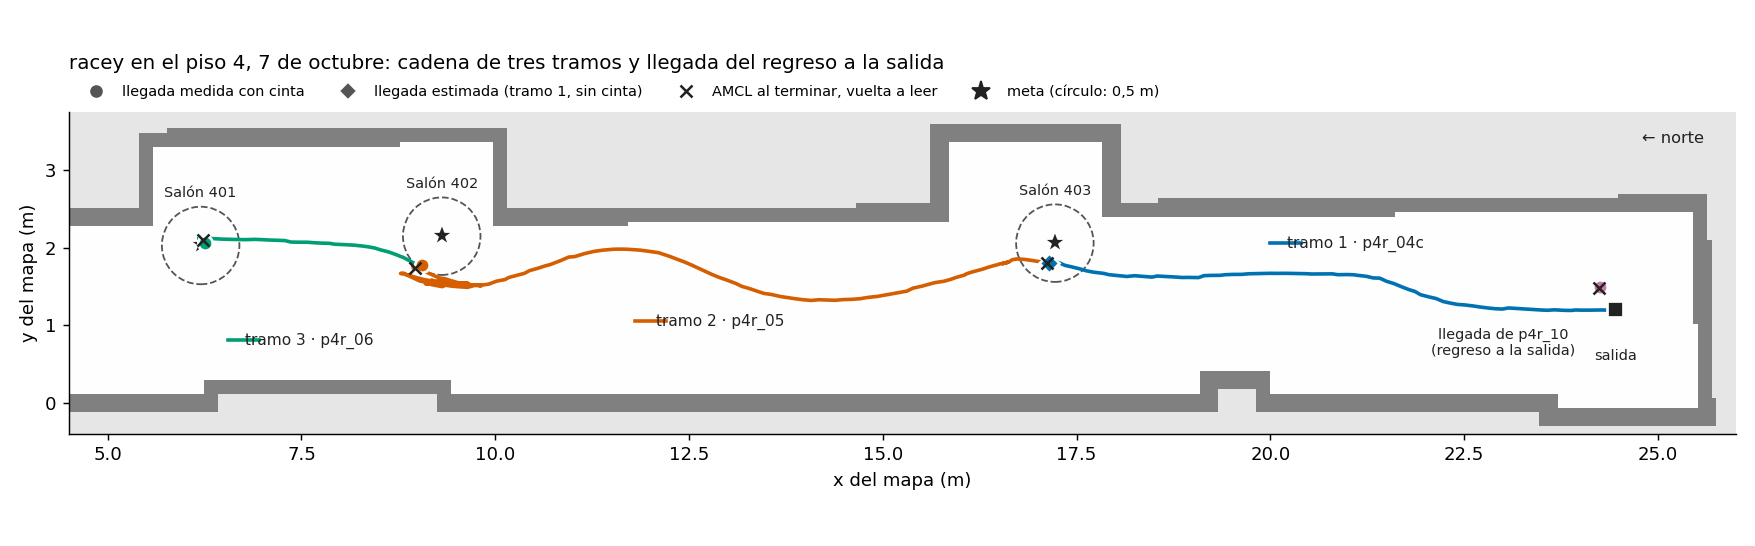
\includegraphics[width=\textwidth]{imagenes/cadena_piso4.png}
  \caption{Cadena de tres tramos en el piso 4 y regreso a la salida: recorrido
    según la localización, llegadas medidas con flexómetro, la llegada estimada
    al Salón 403 y la pose de la localización al terminar cada tramo.}
  \label{fig:cadena}
\end{figure}

Al día siguiente, el otro vehículo recorrió el piso 3 en cinco tramos
encadenados, con dos medias vueltas entre ellos, y los cinco terminaron con éxito
y sin recuperaciones. Esas llegadas no se midieron con flexómetro, y al forzar a la
localización a recalcular su pose al final de cada tramo, esta se desplazó entre 0,61 y 0,86~m. La pose que publica la localización al detenerse el vehículo va atrasada, y por eso la llegada que vale es la medida con flexómetro. Lo que condiciona la precisión de llegada sigue siendo la banda
muerta de tracción (sección~\ref{sec:banda-muerta}): el vehículo se aproxima a la
meta a 0,40~m/s y no tiene régimen de aproximación fina.

% ---------------------------------------------------------------------
\section{Evaluación del sistema completo con los dos vehículos}
\label{sec:res-completo}

El sistema completo funcionó sobre los dos vehículos. La misión con relevo del
Salón 302 al Salón 402 se completó, y de las diez misiones sorteadas para la
campaña, las nueve que llegaron a correr se completaron, todas con relevo. La
décima quedó interrumpida porque el computador portátil se apagó por falta de
batería.

\subsection{Condiciones de las pruebas}

Las pruebas se hicieron en los pisos 3 y 4, con un vehículo en cada piso. El
coordinador y el grabador corrieron en el portátil, y cada misión se pidió desde
la página web en un teléfono conectado a la red de los vehículos. Los autores
hicieron de usuario: pidieron cada misión, acompañaron a los vehículos y
confirmaron el cambio de piso en la página. Los vehículos no se reubicaron entre
misiones, y cuando el destino quedaba detrás del vehículo, el coordinador pidió la
media vuelta en varios tiempos (sección~\ref{sec:media-vuelta}). La llegada se verificó con la localización de cada vehículo y no con flexómetro (sección~\ref{sec:lim-llegada}).

\subsection{La misión con relevo}

La primera prueba del sistema completo fue una misión del Salón 302, en el piso 3,
al Salón 402, en el piso 4. Se completó en 132,5~s, con un relevo y con la llegada
a 0,444~m del destino. Entre la llegada del primer vehículo a la escalera y el
arranque del segundo pasaron 61,1~s. Fue el segundo intento: en el primero, el
coordinador rechazó la llegada del vehículo del piso 3 al Salón 302, adonde iba a
recoger al usuario, porque su localización lo situaba a 0,59~m del punto.

Esa sesión sirvió de ensayo del montaje, y en ella los autores eligieron las
misiones sin seguir el sorteo. De las doce misiones grabadas, siete se completaron
y cinco terminaron fallidas: en cuatro, el coordinador rechazó una llegada con el
vehículo a entre 0,51 y 0,78~m del punto, y en la otra Nav2 abortó la navegación.
Estas misiones no forman parte de la campaña.

\subsection{La campaña con las misiones sorteadas}

Las diez misiones de la campaña se sortearon antes de correr, con una semilla
fija, entre los puntos de interés de los dos pisos: cinco de subida y cinco de
bajada (sección~\ref{sec:pruebas-verificacion}). Corrieron en el orden del
sorteo, y la tabla~\ref{tab:campana-vehiculos} da el resultado de las nueve que
llegaron a correr.

\begin{table}[htbp]
  \centering\small
  \caption{Campaña con los dos vehículos: las nueve misiones sorteadas que
    corrieron, todas completadas con un relevo. La llegada es la de la
    localización del vehículo, con una tolerancia de 0,5~m.}
  \label{tab:campana-vehiculos}
  \begin{tabular}{@{}cllccc@{}}
    \toprule
    \textbf{N.\textsuperscript{o}} & \textbf{Origen} & \textbf{Destino} & \textbf{Tiempo total} & \textbf{Respuesta} & \textbf{Llegada} \\ \midrule
    1 & Ascensor, piso 3 & Salón 403 & 52,3 s & 0,51 s & 0,435 m \\
    2 & Salón 302 & Salón 401 & 90,1 s & 0,27 s & 0,202 m \\
    3 & Salón 401 & Salón 302 & 87,6 s & 3,90 s & 0,143 m \\
    4 & Salón 403 & Salón 303 & 78,9 s & 1,25 s & 0,420 m \\
    5 & Salón 402 & Salón 301 & 105,4 s & 0,66 s & 0,285 m \\
    6 & Salón 301 & Salón 401 & 89,8 s & 2,97 s & 0,226 m \\
    7 & Ascensor, piso 4 & Salón 301 & 81,7 s & 0,87 s & 0,234 m \\
    8 & Salón 302 & Salón 403 & 81,8 s & 0,95 s & 0,214 m \\
    9 & Salón 303 & Salón 402 & 92,6 s & 0,63 s & 0,299 m \\ \midrule
    \multicolumn{3}{@{}l}{Mediana} & 87,6 s & 0,87 s & 0,234 m \\ \bottomrule
  \end{tabular}
\end{table}

Con nueve éxitos en nueve misiones, el intervalo de Wilson al 95~\% va del 70,1 al
100~\%. Lo que podemos afirmar es que la tasa de éxito sobre los vehículos supera
el 70~\%, la misma cota que sostiene la campaña en simulación. Expresado como en
la sección~\ref{sec:teo-evaluacion}, nueve repeticiones sin fallo demuestran una
fiabilidad mínima de 0,81 con un 85~\% de confianza.

El error de llegada tuvo una mediana de 0,234~m y fue de 0,143 a 0,435~m. El
tiempo total, desde la solicitud hasta la llegada verificada, tuvo una mediana de
87,6~s y fue de 52,3 a 105,4~s. El tiempo de respuesta, desde que el coordinador
acepta la solicitud hasta que el vehículo asignado empieza a moverse, tuvo una
mediana de 0,87~s y quedó por debajo de 1,3~s en siete de las nueve misiones. Los
dos valores más altos, 3,90 y 2,97~s, son de misiones en que el vehículo ya estaba
en el punto de origen. El coordinador verificó esa llegada, que no exigía moverse,
con la espera de 1,5~s, y el primer movimiento fue la media vuelta hacia la
escalera. El tiempo de asignación fue de 0,3~ms en las nueve misiones, medido con el reloj del portátil e incluyendo el paso del mensaje hasta el grabador, del mismo orden que el del banco de pruebas
(sección~\ref{sec:res-sim}). En las nueve misiones los vehículos hicieron 24 medias
vueltas, de entre 160 y 171$^\circ$, en uno a cuatro tiempos cada una.

La figura~\ref{fig:campana-vehiculos} descompone el tiempo de cada misión en sus
etapas. Ir a recoger al usuario tomó entre 2,2 y 30,6~s, según dónde había
terminado la misión anterior. El guiado en el piso de origen tuvo una mediana de
24,2~s, y el guiado en el piso de destino, de 24,8~s.

\begin{figure}[htbp]
  \centering
  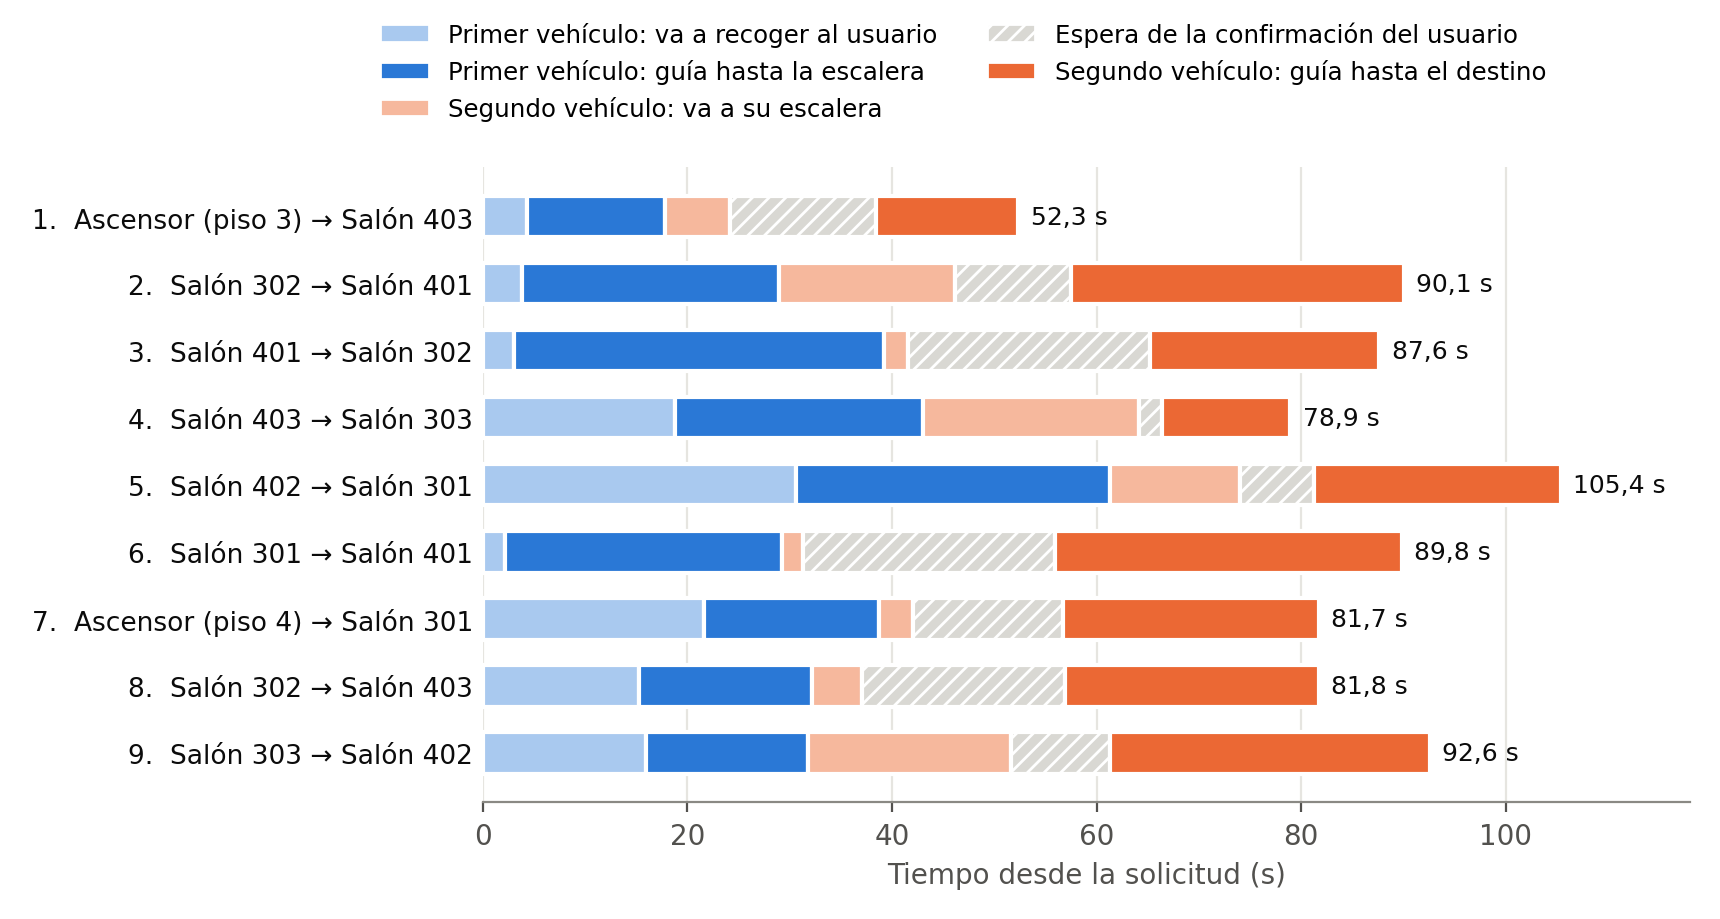
\includegraphics[width=\textwidth]{imagenes/campana_vehiculos_etapas.png}
  \caption{Duración de cada etapa en las nueve misiones de la campaña con los
    vehículos, según las marcas de etapa del coordinador. El tramo rayado es la
    espera de la confirmación de cambio de piso, contada desde que el segundo
    vehículo está en su escalera.}
  \label{fig:campana-vehiculos}
\end{figure}

\subsection{El relevo entre los dos vehículos}

En las nueve misiones el relevo se produjo y el coordinador no pasó por el estado
inactivo ni quedó sin agente asignado. Como en simulación, ese criterio no puede
fallar por la forma en que está construido (sección~\ref{sec:limitaciones}). La medida que informa es el intervalo del relevo: el tiempo desde que el primer
vehículo llega a su escalera hasta el primer movimiento del segundo.

Ese intervalo tuvo una mediana de 1,22~s, pero la cifra junta dos situaciones. En
cinco misiones el segundo vehículo tuvo que desplazarse hasta su escalera, en
cuatro desde el destino de la misión anterior y en una para corregir su posición
unos centímetros, y arrancó en menos de 1,3~s. En las otras cuatro ya estaba en la
escalera, su primer movimiento fue el del guiado final, después de la
confirmación, y el intervalo, de 12,9 a 27,5~s, mide sobre todo cuánto tardó la
persona en confirmar.

Para la persona, lo que cuenta es el tiempo entre la llegada a la escalera del
piso de origen y el arranque del guiado en el piso de destino. En ese tiempo
cambia de piso, el segundo vehículo llega a su escalera si no estaba allí, y la
persona confirma en la página. Tuvo una mediana de 24,8~s y fue de 18,0 a
29,5~s. La confirmación, desde que el segundo vehículo estaba en su escalera, tomó
entre 2,3 y 24,7~s, y el aviso de los 60~s no llegó a mostrarse en ninguna misión.

\subsection{Criterio de conteo e incidencias}

La campaña cuenta, por decisión de los autores, una corrida por misión: la que se
completó. El protocolo, en cambio, cuenta como fallo toda corrida fallida, y por
eso los intentos que no entran en la tasa se declaran aquí. Las misiones 1 y 2 se
completaron en el segundo intento. Los dos primeros intentos fallaron en el tramo
en que el vehículo del piso 3 iba a recoger al usuario. En el de la misión 1, el
coordinador rechazó la llegada al ascensor, con el vehículo a 0,526~m del punto, y
en el de la misión 2 no tenía la pose del vehículo para verificar la llegada.

Antes de esos intentos, la navegación de los dos vehículos dejó de responder.
Ocho intentos de la misión 1 terminaron rechazados o abortados, con las
transformadas de posición detenidas dentro de Nav2. Los dos vehículos llevaban
horas encendidos, con cargas de 10 a 14 en procesadores de dos núcleos. Se
reiniciaron las cadenas de navegación con la pose de salida, y después las nueve
misiones corrieron sin tocar los vehículos. La causa de la detención no se
estableció.

La misión 10 empezó y no terminó: el portátil se apagó por falta de batería unos
30~s después de pedirla, cuando el vehículo del piso 4 ya había llegado a su
escalera. Unos minutos antes se había pedido por error el ascensor del piso 4 como
destino, porque los ascensores de los dos pisos aparecían en la página con el mismo nombre. Ese intento no es una misión del sorteo y no se cuenta. Después de
la campaña, la página muestra el piso junto a los nombres que se repiten
(sección~\ref{sec:ajustes-campo}).

% ---------------------------------------------------------------------
\section{Limitaciones de la medición}
\label{sec:limitaciones}

\subsection{Naturaleza del criterio de continuidad entre niveles}

La continuidad del servicio es la variable de respuesta principal del cuarto
objetivo, y su criterio binario se cumplió en las treinta misiones. Ese resultado,
sin embargo, no es evidencia. El criterio exige que, dentro de la ventana de la
misión, el coordinador nunca esté inactivo ni tenga el agente sin asignar. Los dos únicos puntos del código que producen esos valores ocurren antes de que la
ventana se abra. No existe ejecución posible que lo incumpla, y un criterio que no
puede dar resultado negativo no aporta evidencia, por muchas veces que se
verifique \autocite{popper1959logic}.

No quisimos corregirlo inventando una ruta de fallo, porque eso habría sido
instrumentar el experimento para que pareciera más informativo. La continuidad
se declaró como un invariante estructural del diseño, y la afirmación se apoyó en
una magnitud que sí varía: el intervalo del relevo, entre el final del tramo de un
vehículo y el inicio del tramo del otro. En las quince misiones entre pisos tuvo
una mediana de 0,1~s y un máximo de 0,2~s, es decir, uno o dos pasos del reloj de
la simulación.

\subsection{Espacio desconocido marcado como libre en el mapa}

El mapa con que corrió la campaña en simulación declaraba un umbral que hacía que
10\,908 celdas desconocidas, el 14,5~\% del mapa, se cargaran como espacio libre.
Con ello quedaban desactivadas en la práctica las dos salvaguardas que debían
impedir planificar sobre lo no explorado. Esto no invalida el veredicto de la
campaña: los cuatro fallos fueron de precisión de llegada, no de trazado, y el
pasillo por el que se navegó está libre en el mundo real. Lo que no se sabe es si
alguna trayectoria cruzó una de esas celdas, algo comprobable sobre los registros
conservados. El defecto se corrigió después de la campaña.

\subsection{La llegada en los vehículos, sin medida externa}
\label{sec:lim-llegada}

En la campaña con los vehículos la llegada no tuvo una medida independiente del
sistema. El protocolo la toma con flexómetro sobre marcas en el piso, y en esa
sesión no se midió. El error que se reporta es el de la localización del propio
vehículo contra el punto del catálogo, leído 1,5~s después de que Nav2 diera la
meta por alcanzada, con el vehículo ya detenido. Es la medida con que el coordinador acepta la llegada, así que el sistema verificó su llegada con su
propia estimación, que es lo que la regla principal del protocolo procura evitar
(sección~\ref{sec:protocolo}). Los registros lo declaran con la procedencia de la
medida, y el analizador lo advierte al calcular las métricas.

La única comparación entre la localización y el flexómetro en los vehículos es la
de la cadena de tres tramos en el piso 4 (sección~\ref{sec:res-g3}). Leída de
nuevo al terminar cada tramo, la localización quedó a 0,10~m o menos de la medida
en el sentido del avance y a 5~cm o menos de lado. En el piso 3, en cambio, forzar
a la localización a recalcular su pose al final de cada tramo la desplazó entre
0,61 y 0,86~m. Por eso leemos el resultado de la campaña así: cada vehículo,
según su propia localización, llegó a menos de 0,5~m del destino. Que la
distancia real cumpliera la misma tolerancia no está medido.
